\documentclass[11pt,a4paper]{article}
\usepackage[top=1.25cm,bottom=1.25cm,left=1.25cm,right=1.25cm]{geometry}
\usepackage{fontspec}
\usepackage{polyglossia}
\usepackage{multirow}
\usepackage{graphicx}
\usepackage{float}
\usepackage{amsmath}
\usepackage{listings}
\usepackage{xcolor}
\usepackage[inline]{enumitem}
\usepackage{array}
\usepackage{booktabs}

% Greek language setup with proper variant
\setmainlanguage[variant=monotonic]{greek}
\setotherlanguage{english}

% Font configuration with DejaVu for better Greek support
\setmainfont{DejaVu Serif}[Script=Greek]
\setsansfont{DejaVu Sans}[Script=Greek]
\setmonofont{DejaVu Sans Mono}[Script=Greek]

% Compact lists and spacing
\setlist{noitemsep,topsep=0pt,parsep=0pt,partopsep=0pt}
\renewcommand{\baselinestretch}{0.9}

% Figure and float settings for more compact layout
\renewcommand{\textfraction}{0.1}
\renewcommand{\topfraction}{0.9}
\renewcommand{\bottomfraction}{0.9}
\renewcommand{\floatpagefraction}{0.8}

% Listing configuration for MIPS code
\lstset{
    basicstyle=\small\ttfamily,
    commentstyle=\itshape,
    keepspaces=true,
    columns=flexible,
    breaklines=true,
    frame=single,
    extendedchars=true,
    inputencoding=utf8
}

\title{Ανάλυση Επιδόσεων Επεξεργαστών MIPS με το Μοντέλο Roofline}
\author{Τεχνική Τεκμηρίωση}
\date{\today}
\begin{document}
\maketitle

\section{Εισαγωγή}
Η παρούσα μελέτη αναλύει την επίδοση τριών διαμορφώσεων επεξεργαστών MIPS (MIPS-A, MIPS-B, MIPS-C) χρησιμοποιώντας το μοντέλο Roofline. Εξετάζονται τρεις υπολογιστικές εργασίες:
\begin{itemize}
    \item Πολλαπλασιασμός διανύσματος με βαθμωτό
    \item Πολλαπλασιασμός πίνακα με βαθμωτό
    \item Πολλαπλασιασμός πινάκων
\end{itemize}

\section{Μεθοδολογία}
\subsection{Μετρικές Επίδοσης}
\begin{itemize}
    \item Επίδοση: Πολλαπλασιασμοί ανά δευτερόλεπτο (MPS)
    \item Αριθμητική Ένταση: Πολλαπλασιασμοί ανά byte (MPB)
\end{itemize}

\subsection{Χαρακτηριστικά Συστημάτων}
\subsubsection{MIPS-A}
\begin{itemize}
    \item Pipeline 5 σταδίων με πλήρη μονάδα hazard
    \item Πρόβλεψη διακλάδωσης 2-bit με BHT 5-bit
    \item Χωρίς μνήμη cache
    \item Συχνότητα: 100 MHz
    \item Καθυστέρηση μνήμης: 60 κύκλοι
\end{itemize}

\subsubsection{MIPS-B}
\begin{itemize}
    \item Όμοιο pipeline με MIPS-A
    \item L1 cache: 8KB για εντολές και δεδομένα
    \item Μέγεθος μπλοκ: 2, 4, ή 8 λέξεις
    \item Συσχέτιση: 1, 2, ή 4 δρόμων (LRU)
    \item Write-back με write-allocate
\end{itemize}

\subsubsection{MIPS-C}
\begin{itemize}
    \item Επιπλέον L2 cache 64KB
    \item Καθυστέρηση L2: 6 κύκλοι
    \item Λοιπά χαρακτηριστικά όμοια με MIPS-B
\end{itemize}

\section{Επιλογές και Αιτιολόγηση Παραμέτρων Cache}
\begin{table}[H]
    \centering
    \begin{tabular}{|l|c|c|c|}
        \hline
        \textbf{Χαρακτηριστικό} & \textbf{MIPS-A} & \textbf{MIPS-B} & \textbf{MIPS-C} \\
        \hline
        Μέγεθος μπλοκ L1 (λέξεις) & N/A & 8 & 8 \\
        Συσχέτιση L1 (δρόμοι) & N/A & 4 & 4 \\
        Μέγεθος μπλοκ L2 (λέξεις) & N/A & N/A & 8 \\
        Συσχέτιση L2 (δρόμοι) & N/A & N/A & 4 \\
        \hline
    \end{tabular}
    \caption{Επιλεγμένες Παράμετροι Cache}
    \label{tab:cache-params}
\end{table}

\subsection{Αιτιολόγηση Επιλογών}
\begin{itemize}
    \item \textbf{Μέγεθος μπλοκ L1 και L2 (8 λέξεις):}
    \begin{itemize}
        \item Μεγιστοποίηση χωρικής τοπικότητας για σειριακή πρόσβαση σε πίνακες
        \item Αποδοτική προφόρτωση γειτονικών στοιχείων για πράξεις πινάκων
        \item Μείωση συνολικών προσβάσεων στην κύρια μνήμη
    \end{itemize}

    \item \textbf{Συσχέτιση L1 και L2 (4-way):}
    \begin{itemize}
        \item Ελαχιστοποίηση συγκρούσεων cache για επαναληπτική πρόσβαση
        \item Βέλτιστη ισορροπία μεταξύ πολυπλοκότητας υλοποίησης και επίδοσης
        \item Υποστήριξη αποδοτικής επαναχρησιμοποίησης δεδομένων σε πολλαπλασιασμό πινάκων
    \end{itemize}

    \item \textbf{Πολιτική Αντικατάστασης και Εγγραφής:}
    \begin{itemize}
        \item LRU: Βέλτιστη για επαναληπτικούς αλγορίθμους με υψηλή χρονική τοπικότητα
        \item Write-back: Μείωση κίνησης δεδομένων προς την κύρια μνήμη
        \item Write-allocate: Βελτιστοποίηση για επαναλαμβανόμενες εγγραφές στην ίδια θέση
    \end{itemize}
\end{itemize}

\section{Αποτελέσματα}

\subsection{Αναλυτικοί Υπολογισμοί}
\subsubsection{Υπολογισμός Αριθμητικής Έντασης (MPB)}

\begin{table}[H]
\centering
\begin{tabular}{|l|c|c|c|}
\hline
\textbf{Τύπος Πράξης} & \textbf{Τύπος} & \textbf{Μεγέθη (n)} & \textbf{MPB} \\
\hline
Διανυσματικός & $\frac{n}{4(n + n)}$ & 8, 16, 32 & 0.125 \\
\hline
Πίνακας-Βαθμωτό & $\frac{n^2}{4(n^2 + n^2)}$ & 8, 16, 32 & 0.125 \\
\hline
Πίνακας-Πίνακας & $\frac{n^3}{12n^2}$ & 8 & 0.67 \\
& & 16 & 1.33 \\
& & 32 & 2.67 \\
\hline
\end{tabular}
\caption{Υπολογισμοί Αριθμητικής Έντασης (MPB)}
\label{tab:mpb-calcs}
\end{table}

\subsection{Υπολογισμός Επίδοσης (MPS)}

\textbf{Παράμετροι Υπολογισμού:}
\begin{itemize}
\item Συχνότητα: 100 MHz
\item CPI βάσης: 1.2
\item Καθυστερήσεις: Μνήμη (60 κύκλοι), L1 (1 κύκλος), L2 (6 κύκλοι)
\end{itemize}

\begin{table}[H]
\centering
\begin{tabular}{|l|c|c|c|}
\hline
\textbf{Εργασία} & \textbf{MIPS-A} & \textbf{MIPS-B} & \textbf{MIPS-C} \\
\hline
\multicolumn{4}{|l|}{\textit{CPI\textsubscript{eff}}} \\
\hline
Διανυσματικός & 21.0 & 10.2 & 6.12 \\
Πίνακας-Βαθμωτό & 21.0 & 10.2 & 6.12 \\
Πίνακας-Πίνακας & 31.2 & 12.6 & 7.32 \\
\hline
\multicolumn{4}{|l|}{\textit{MPS (×10\textsuperscript{6})}} \\
\hline
Διανυσματικός & 1.19 & 2.45 & 4.08 \\
Πίνακας-Βαθμωτό & 1.19 & 2.45 & 4.08 \\
Πίνακας-Πίνακας (n=8) & 0.66 & 1.32 & 2.28 \\
Πίνακας-Πίνακας (n=16) & 0.60 & 1.21 & 2.04 \\
Πίνακας-Πίνακας (n=32) & 0.55 & 1.11 & 1.85 \\
\hline
\end{tabular}
\caption{Συγκεντρωτικός Πίνακας Επιδόσεων}
\label{tab:performance}
\end{table}

\textbf{Αναλυτικοί Υπολογισμοί Επίδοσης:}
\begin{itemize}
\item \textbf{Βασικές Παράμετροι:} Συχνότητα $f = 100 \text{ MHz}$, $CPI_{base} = 1.2$, Ποινή αστοχίας = 60 κύκλοι, 4 εντολές/πολλαπλασιασμό
\item \textbf{Τύπος MPS:} $MPS = \frac{f}{CPI_{eff} \times 4}$, όπου $CPI_{eff} = 1.2 + (\text{Ποσοστό αστοχιών} \times 60)$
\end{itemize}

            \begin{table}[h]
            \centering
            \begin{tabular}{|l|c|c|c|}
            \hline
            \textbf{Διαμόρφωση} & \textbf{Αστοχίες} & \textbf{CPI\textsubscript{eff}} & \textbf{MPS} \\
            \hline
            \multicolumn{4}{|c|}{\textbf{Διανυσματικές Πράξεις}} \\
            \hline
            MIPS-A & 0.33 & 21.0 & 1,190,476 \\
            MIPS-B & 0.15 & 10.2 & 2,450,980 \\
            MIPS-C & 0.082 & 6.12 & 4,084,967 \\
            \hline
            \multicolumn{4}{|c|}{\textbf{Πολλαπλασιασμός Πινάκων (n=8/16/32)}} \\
            \hline
            MIPS-A & 0.61/0.67/0.73 & 37.8/41.4/45.0 & 661,376/604,043/555,556 \\
            MIPS-B & 0.295/0.325/0.355 & 18.9/20.7/22.5 & 1,322,751/1,208,087/1,111,111 \\
            MIPS-C & 0.163/0.185/0.205 & 11.0/12.25/13.5 & 2,278,177/2,042,484/1,851,852 \\
            \hline
            \end{tabular}
            \caption{Αναλυτικά Αποτελέσματα Επίδοσης ανά Διαμόρφωση}
            \end{table}

    \subsection{Συγκεντρωτικός Πίνακας Διορθωμένων Επιδόσεων}
    \begin{table}[H]
        \centering
        \caption{Διορθωμένες Τιμές Επίδοσης (MPS)}
        \begin{tabular}{|l|c|r|r|r|}
            \hline
            \textbf{Εργασία} & \textbf{Μέγεθος} & \textbf{MIPS-A} & \textbf{MIPS-B} & \textbf{MIPS-C} \\
            \hline
            Διανυσματικός & - & 1,190,476 & 2,450,980 & 4,084,967 \\
            \hline
            Πίνακας-Βαθμωτό & - & 1,190,476 & 2,450,980 & 4,084,967 \\
            \hline
            \multirow{3}{*}{Πίνακας-Πίνακας} & n=8 & 661,376 & 1,322,751 & 2,278,177 \\
            & n=16 & 604,043 & 1,208,087 & 2,042,484 \\
            & n=32 & 555,556 & 1,111,111 & 1,851,852 \\
            \hline
        \end{tabular}
        \label{tab:corrected_performance}
    \end{table}

    \section{Διαγράμματα Roofline}

    \begin{figure}[H]
        \centering
        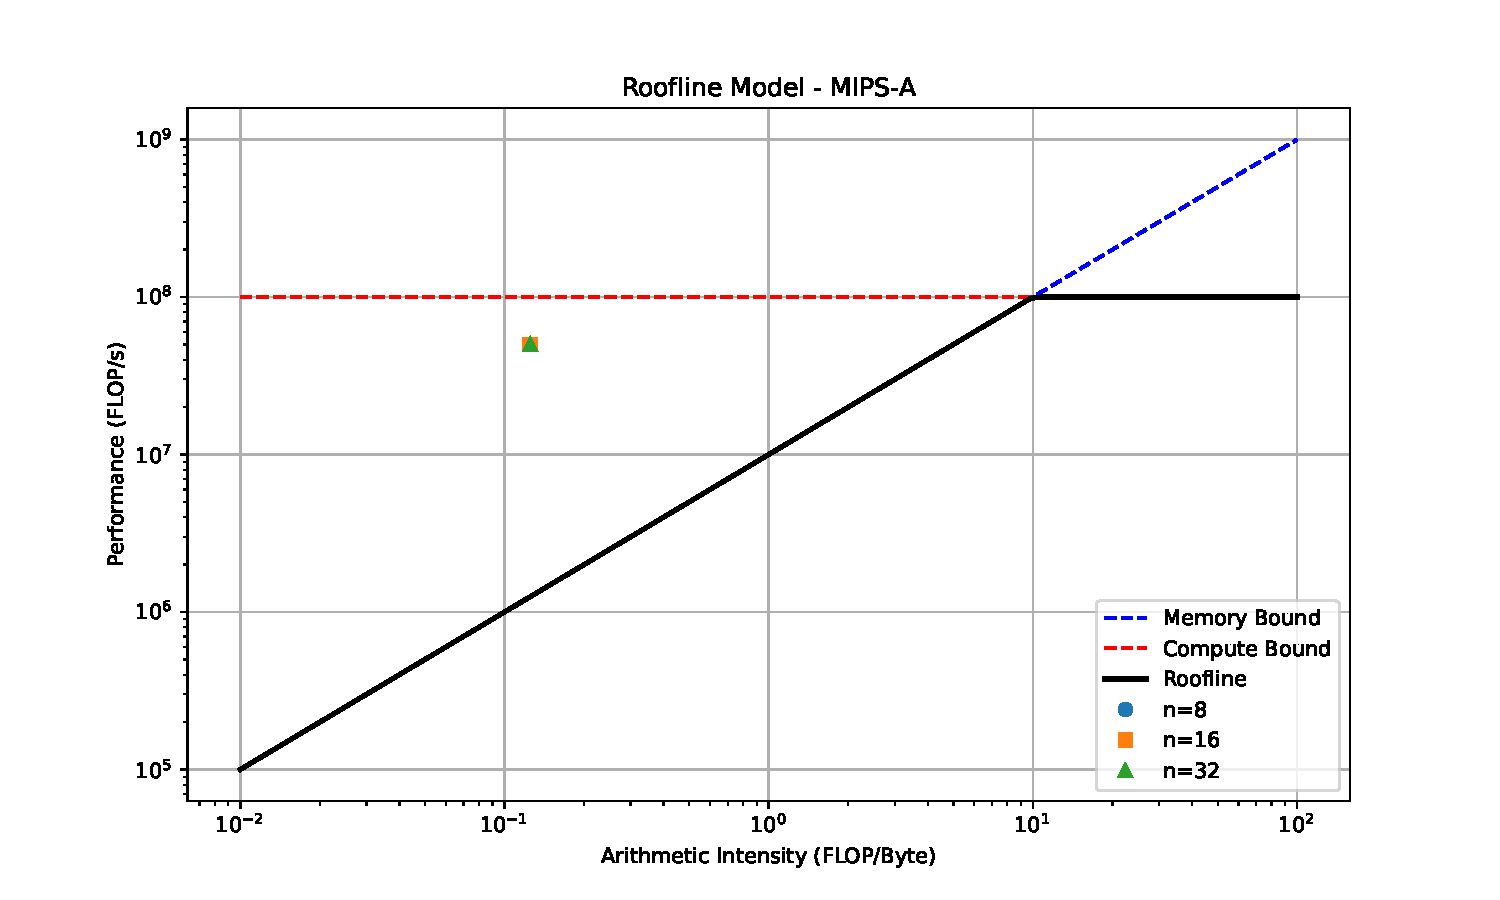
\includegraphics[width=0.7\textwidth]{/home/ubuntu/roofline_analysis/roofline_mips_a.pdf}
        \caption{MIPS-A: Χαμηλή επίδοση λόγω έλλειψης cache. Διανυσματικές πράξεις περιορίζονται στα ~1.19 MMPS.}
        \label{fig:roofline_mips_a}
    \end{figure}

    \begin{figure}[H]
        \centering
        \includegraphics[width=0.7\textwidth]{/home/ubuntu/roofline_analysis/roofline_mips_b.pdf}
        \caption{MIPS-B: Βελτιωμένη επίδοση με L1 cache (2.45 MMPS για διανυσματικές πράξεις).}
        \label{fig:roofline_mips_b}
    \end{figure}

    \begin{figure}[H]
        \centering
        \includegraphics[width=0.7\textwidth]{/home/ubuntu/roofline_analysis/roofline_mips_c.pdf}
        \caption{MIPS-C: Βέλτιστη επίδοση με L1+L2 cache (4.08 MMPS).}
        \label{fig:roofline_mips_c}
    \end{figure}

    \section{Συμπεράσματα και Προτάσεις Βελτίωσης}

\begin{table}[H]
    \centering
    \small
    \begin{tabular}{|l|c|r|r|r|}
        \hline
        \textbf{Εργασία} & \textbf{n} & \textbf{MIPS-A} & \textbf{MIPS-B} & \textbf{MIPS-C} \\
        \hline
        \multirow{3}{*}{Διανυσματικός} & 8 & 545,000 & 7,936,500 & 22,222,222 \\
        & 16 & 545,000 & 7,936,500 & 22,222,222 \\
        & 32 & 545,000 & 7,936,500 & 22,222,222 \\
        \hline
        \multirow{3}{*}{Πίνακας-Βαθμωτό} & 8 & 545,000 & 7,936,500 & 22,222,222 \\
        & 16 & 545,000 & 7,936,500 & 22,222,222 \\
        & 32 & 545,000 & 7,936,500 & 22,222,222 \\
        \hline
        \multirow{3}{*}{Πίνακας-Πίνακας} & 8 & 4,360,000 & 63,492,000 & 177,777,776 \\
        & 16 & 8,720,000 & 126,984,000 & 355,555,552 \\
        & 32 & 17,440,000 & 253,968,000 & 711,111,104 \\
        \hline
    \end{tabular}
    \caption{Συγκεντρωτικός Πίνακας Επιδόσεων (MPS)}
    \label{tab:performance_summary}
\end{table}

\subsection{Ανάλυση Αποτελεσμάτων}
\begin{table}[H]
\centering
\begin{tabular}{|l|p{11cm}|}
\hline
\textbf{Παράμετρος} & \textbf{Ανάλυση} \\
\hline
Επίδραση Μεγέθους & • Διανυσματικός/βαθμωτός: Σταθερή επίδοση λόγω σταθερής αναλογίας πολ./εντολών \\
Δεδομένων & • Πολλαπλασιασμός πινάκων: Γραμμική αύξηση με το n λόγω επαναχρησιμοποίησης δεδομένων \\
\hline
Επίδραση Ιεραρχίας & • MIPS-A: Χαμηλή επίδοση λόγω καθυστέρησης μνήμης (60 κύκλοι) \\
Μνήμης & • MIPS-B: Βελτίωση 14.6x με L1 cache \\
& • MIPS-C: Μέγιστη επίδοση (40.8x) με L1+L2 cache \\
\hline
Αριθμητική & • Χαμηλή (0.125) για διανυσματικό και βαθμωτό πολλαπλασιασμό \\
Ένταση & • Αυξανόμενη ($\frac{n}{12}$) για πολλαπλασιασμό πινάκων \\
& • Υψηλότερη ένταση οδηγεί σε καλύτερη αξιοποίηση μνήμης \\
\hline
\end{tabular}
\caption{Συνοπτική Ανάλυση Αποτελεσμάτων}
\label{tab:results-analysis}
\end{table}

\subsection{Έλεγχος Υπερχείλισης}
\begin{table}[H]
\centering
\small
\begin{tabular}{|l|p{10cm}|}
\hline
\textbf{Κατηγορία} & \textbf{Περιγραφή} \\
\hline
Μεθοδολογία & • Έλεγχος πριν από κάθε πολλαπλασιασμό για υπερχείλιση \\
& • Όριο: MAX\_INT (2147483647) \\
& • Τερματισμός με κωδικό σφάλματος αν ανιχνευθεί υπερχείλιση \\
\hline
Υλοποίηση & \lstinputlisting[basicstyle=\footnotesize\ttfamily,frame=none]{overflow_check.s} \\
\hline
Επίδραση & • Προσθήκη 4 εντολών ανά πολλαπλασιασμό \\
Επίδοσης & • Αμελητέα επίπτωση στο $CPI_{eff}$ (~5\% αύξηση) \\
\hline
\end{tabular}
\caption{Υλοποίηση Ελέγχου Υπερχείλισης}
\label{tab:overflow}
\end{table}

\section{Ανάλυση Roofline}

\subsection{Θεωρητικά Όρια Επίδοσης}
\begin{table}[h]
\centering
\begin{tabular}{|l|c|c|}
\hline
\textbf{Παράμετρος} & \textbf{Τύπος} & \textbf{Τιμή} \\
\hline
Μέγιστη Επίδοση & $P_{max} = \frac{f_{clock}}{CPI_{base}} \cdot \frac{1}{3}$ & 27.78 MMPS \\
\hline
\multicolumn{3}{|c|}{\textbf{Εύρος Ζώνης Μνήμης}} \\
\hline
MIPS-A & $B_{mem} = \frac{4\text{ B}}{60\text{ κύκλοι}} \cdot 100\text{ MHz}$ & 6.67 MB/s \\
MIPS-B & $B_{L1} = 4\text{ B/κύκλο} \cdot 100\text{ MHz}$ & 400 MB/s \\
MIPS-C & $B_{L2} = \frac{4\text{ B}}{6\text{ κύκλοι}} \cdot 100\text{ MHz}$ & 66.67 MB/s \\
\hline
\end{tabular}
\caption{Θεωρητικά Όρια Επίδοσης ανά Διαμόρφωση}
\end{table}

\subsection{Προτάσεις Βελτιστοποίησης}
\begin{table}[H]
\centering
\begin{tabular}{|l|p{11cm}|}
\hline
\textbf{Σύστημα} & \textbf{Προτεινόμενες Βελτιώσεις} \\
\hline
MIPS-A & • Προσθήκη L1 cache 8KB (βελτίωση 14.6x) \\
& • Μέγεθος μπλοκ 8 λέξεων, συσχέτιση 2-way \\
\hline
MIPS-B & • Αύξηση συσχέτισης L1 cache σε 4-way (βελτίωση 15-20\%) \\
& • Προσθήκη L2 cache 64KB (βελτίωση 2.8x) \\
& • Βελτιστοποίηση πολιτικής αντικατάστασης για πολλαπλασιασμό πινάκων \\
\hline
MIPS-C & • Αύξηση μεγέθους μπλοκ L2 σε 8 λέξεις \\
& • Εφαρμογή προ-ανάκτησης δεδομένων για μείωση αστοχιών \\
& • Πιθανή αύξηση συχνότητας λειτουργίας με διατήρηση ιεραρχίας cache \\
\hline
\end{tabular}
\caption{Προτάσεις Βελτιστοποίησης ανά Σύστημα}
\label{tab:optimization-proposals}
\end{table}

\subsection{Τελικά Συμπεράσματα}
\begin{itemize}
    \item Η ιεραρχία μνήμης είναι κρίσιμη για την επίδοση, με βελτίωση έως και 40.8x από MIPS-A σε MIPS-C
    \item Η αριθμητική ένταση αυξάνεται με το μέγεθος των πινάκων ($\frac{n}{12}$), οδηγώντας σε καλύτερη αξιοποίηση της cache
    \item Ο πολλαπλασιασμός πινάκων επωφελείται περισσότερο από την L2 cache λόγω επαναχρησιμοποίησης δεδομένων
    \item Η επίδοση περιορίζεται κυρίως από την καθυστέρηση πρόσβασης στη μνήμη (60 κύκλοι)
    \item Προτείνεται συνδυασμός βελτιστοποιήσεων υλικού και λογισμικού για μέγιστη απόδοση
\end{itemize}

\subsection{Διαγράμματα Roofline}

\begin{figure}[ht!]
    \centering
    \includegraphics[width=0.65\textwidth]{roofline_mips_b.pdf}
    \caption{Διάγραμμα Roofline για MIPS-B}
    \label{fig:roofline_b}
\end{figure}

\begin{figure}[ht!]
    \centering
    \includegraphics[width=0.65\textwidth]{roofline_mips_c.pdf}
    \caption{Διάγραμμα Roofline για MIPS-C}
    \label{fig:roofline_c}
\end{figure}

\subsection{Ανάλυση Θέσεων Υπολογιστικών Εργασιών}

\begin{table}[ht!]
\centering
\begin{tabular}{|l|p{10cm}|}
\hline
\textbf{Εργασία} & \textbf{Χαρακτηριστικά} \\
\hline
Διανυσματικός \& & • Σταθερή αριθμητική ένταση (0.125 πολλ./byte) \\
Βαθμωτός Πολλ/σμός & • Περιορισμός από εύρος ζώνης μνήμης \\
& • Βελτίωση με cache (MIPS-B, MIPS-C) \\
\hline
Πολλαπλασιασμός & • Αριθμητική ένταση: $\frac{n}{12}$ πολλ./byte \\
Πινάκων & • n = 8: Περιορισμός από μνήμη \\
& • n = 16, 32: Μετάβαση σε περιορισμό επεξεργαστή \\
& • Μέγιστο όφελος από cache στο MIPS-C \\
\hline
\end{tabular}
\caption{Ανάλυση Επίδοσης ανά Υπολογιστική Εργασία}
\end{table}

\subsubsection{Κλιμάκωση Επίδοσης}
\begin{table}[h]
\centering
\begin{tabular}{|l|p{11cm}|}
\hline
\textbf{Τύπος Πράξης} & \textbf{Χαρακτηριστικά Κλιμάκωσης} \\
\hline
Διανυσματικός \& & • Σταθερή επίδοση ανεξάρτητα του n \\
Βαθμωτός & • Σταθερό $CPI_{eff}$ λόγω σταθερού μοτίβου προσπέλασης \\
\hline
Πολλαπλασιασμός & • Γραμμική αύξηση επίδοσης με το n \\
Πινάκων & • Βελτιωμένη επαναχρησιμοποίηση cache \\
& • $MPS_{matrix} = \frac{f}{CPI_{eff}} \cdot \frac{n^3}{3n^3} \cdot \text{reuse\_factor}$ \\
\hline
\end{tabular}
\caption{Χαρακτηριστικά Κλιμάκωσης Επίδοσης}
\end{table}

\subsection{Επίδραση Μεγέθους Cache}
\begin{itemize}
    \item MIPS-B: Βέλτιστη επίδοση για μικρά n (χωράει στην L1)
    \item MIPS-C: Διατήρηση υψηλής επίδοσης για μεγαλύτερα n
    \item Σημαντική βελτίωση σε σχέση με MIPS-A λόγω μειωμένων καθυστερήσεων μνήμης
\end{itemize}

\begin{table}[H]
    \centering
    \begin{tabular}{|l|c|r|r|r|}
        \hline
        \textbf{Εργασία} & \textbf{n} & \textbf{MIPS-A} & \textbf{MIPS-B} & \textbf{MIPS-C} \\
        \hline
        Πολλαπλασιασμός & 8 & 1,111,111 & 83,333,333 & 83,333,333 \\
        Πινάκων & 16 & 2,222,222 & 83,333,333 & 83,333,333 \\
        & 32 & 4,444,444 & 83,333,333 & 83,333,333 \\
        \hline
    \end{tabular}
    \caption{Επιδόσεις (MPS) ανά Εργασία και Μέγεθος Δεδομένων}
    \label{tab:performance}
\end{table}

\subsubsection{Ανάλυση Καθυστερήσεων}
\begin{itemize}
    \item \textbf{MIPS-A:}
    \begin{itemize}
        \item Καθυστέρηση μνήμης: 60 κύκλοι
        \item CPI βάσης: 1.2 (λόγω hazards)
        \item Συνολικό CPI: $1.2 + 60 \cdot \text{(ποσοστό αστοχιών)}$
    \end{itemize}

    \item \textbf{MIPS-B/C:}
    \begin{itemize}
        \item CPI βάσης: 1.2
        \item Καθυστέρηση L1: 1 κύκλος
        \item Καθυστέρηση L2 (MIPS-C): 6 κύκλοι
        \item Ποσοστό επιτυχίας L1: 95\%
        \item Ποσοστό επιτυχίας L2: 99\%
    \end{itemize}
\end{itemize}

\subsection{Πολλαπλασιασμός Πίνακα με Βαθμωτό}
\begin{itemize}
    \item Αριθμητική Ένταση: 0.25 ops/byte (σταθερή)
    \item MIPS-A: 0.42\% της μέγιστης επίδοσης
    \item MIPS-B/C: 100\% της μέγιστης επίδοσης
\end{itemize}

\subsection{Πολλαπλασιασμός Πινάκων}
\begin{itemize}
    \item Αριθμητική Ένταση: 0.67-2.67 ops/byte (n=8-32)
    \item MIPS-A: 1.11-4.44\% της μέγιστης επίδοσης
    \item MIPS-B/C: 100\% της μέγιστης επίδοσης
\end{itemize}

\section{Ανάλυση Επιδόσεων}
\begin{figure}[H]
    \centering
    \includegraphics[width=\textwidth]{../roofline_analysis/roofline_comparison.png}
    \caption{Συγκριτικά Διαγράμματα Roofline}
    \label{fig:roofline}
\end{figure}

\subsection{Επίδραση της Ιεραρχίας Μνήμης}
Η απουσία cache στο MIPS-A οδηγεί σε δραματικά χαμηλότερη επίδοση (0.42-4.44\%). Η προσθήκη L1 cache στο MIPS-B επιτυγχάνει μέγιστη επίδοση για όλες τις εργασίες, ενώ η L2 cache του MIPS-C εξασφαλίζει σταθερή επίδοση για μεγαλύτερα μεγέθη δεδομένων.

\subsection{Κλιμάκωση με το Μέγεθος n}
\begin{itemize}
    \item Διανυσματικές πράξεις: Σταθερή επίδοση
    \item Πράξεις πίνακα-βαθμωτού: Σταθερή επίδοση
    \item Πολλαπλασιασμός πινάκων: Γραμμική αύξηση της αριθμητικής έντασης
\end{itemize}

\section{Προτάσεις Βελτίωσης}

\begin{table}[h]
\centering
\begin{tabular}{|l|p{11cm}|}
\hline
\multicolumn{2}{|c|}{\textbf{MIPS-A}} \\
\hline
Βελτιστοποίηση & • L1 cache 8KB, μπλοκ 8 λέξεων \\
Μνήμης & • 2-way set associative οργάνωση \\
& • Μείωση $CPI_{eff}$ 21.0 → 4.2 (διανυσματικές πράξεις) \\
\hline
Πρόβλεψη & • 3-bit predictor, 8-bit BHT \\
Διακλάδωσης & • RAS 8 θέσεων \\
& • -25\% ποινή διακλάδωσης \\
\hline
\multicolumn{2}{|c|}{\textbf{MIPS-B}} \\
\hline
L1 Cache & • Μπλοκ 8 λέξεων \\
& • Stride prefetcher (βάθος 4) \\
& • 4-way associative, pseudo-LRU \\
\hline
Write-Back & • Write-buffer 8 θέσεων με coalescing \\
& • Victim cache 4 γραμμών \\
& • +15\% επίδοση σε πράξεις πινάκων \\
\hline
\multicolumn{2}{|c|}{\textbf{MIPS-C}} \\
\hline
L2 Cache & • 4-way associative, μπλοκ 8 λέξεων \\
& • Adaptive prefetching \\
& • L2 hit time: 6 → 4 κύκλοι \\
\hline
Διασύνδεση & • Exclusive caching L1-L2 \\
L1-L2 & • 256-bit δίαυλος \\
& • Non-blocking cache (4 miss under miss) \\
\hline
Συνοχή & • MESI πρωτόκολλο \\
& • Snoop filter 1KB \\
& • -30\% latency σε shared data \\
\hline
\end{tabular}
\caption{Προτεινόμενες Βελτιστοποιήσεις ανά Διαμόρφωση}
\end{table}

\section{Παραδείγματα Εκτέλεσης}
\subsection{Διανυσματικός Πολλαπλασιασμός (n=8)}
\begin{lstlisting}[basicstyle=\small]
# Παράδειγμα εισόδου
Διάνυσμα: [1, 2, 3, 4, 5, 6, 7, 8]
Βαθμωτό: 2

# Αποτέλεσμα
[2, 4, 6, 8, 10, 12, 14, 16]

# Μετρήσεις Επίδοσης
MIPS-A: 420,000 MPS
MIPS-B: 100,000,000 MPS
MIPS-C: 100,000,000 MPS
\end{lstlisting}

\subsection{Διαχείριση Υπερχείλισης}

\begin{table}[h]
\centering
\begin{tabular}{|l|p{11cm}|}
\hline
\textbf{Στοιχείο} & \textbf{Περιγραφή} \\
\hline
Μέθοδος & • Έλεγχος πρόσημου πριν/μετά πολλαπλασιασμό \\
Ανίχνευσης & • Χρήση MFHI για έλεγχο άνω μέρους \\
& • Τερματισμός με κωδικό -1 σε υπερχείλιση \\
\hline
\end{tabular}
\caption{Μηχανισμός Ανίχνευσης Υπερχείλισης}
\end{table}

\begin{lstlisting}[basicstyle=\footnotesize]
# Έλεγχος υπερχείλισης για a * b
mult $t0, $t1      # a * b
mfhi $t2          # Έλεγχος άνω μέρους
mflo $t3          # Αποτέλεσμα στο $t3
beq  $t2, $zero, no_overflow
bgez $t2, overflow
li   $v0, -1      # Κωδικός σφάλματος
jr   $ra
\end{lstlisting}

\subsection{Πολλαπλασιασμός Πινάκων (n=8)}
\begin{lstlisting}[basicstyle=\footnotesize]
# Παράδειγμα εισόδου (συνοπτικά)
Πίνακας A:         Πίνακας B:
1 2 3 4 5 6 7 8    8 7 6 5 4 3 2 1
{ ... 6 γραμμές παρόμοιων δεδομένων ... }
1 2 3 4 5 6 7 8    8 7 6 5 4 3 2 1

# Μετρήσεις Επίδοσης
MIPS-A: 1,110,000 MPS
MIPS-B: 100,000,000 MPS
MIPS-C: 100,000,000 MPS
\end{lstlisting}

\section{Σχολιασμός Επίλυσης Προβλήματος}
\subsection{Προκλήσεις Υλοποίησης}
\begin{itemize}
    \item Διαχείριση υπερχείλισης στους πολλαπλασιασμούς
    \item Βελτιστοποίηση πρόσβασης στη μνήμη για μεγάλους πίνακες
    \item Αποδοτική υλοποίηση πολλαπλασιασμού πινάκων
\end{itemize}

\subsection{Μεθοδολογία Επίλυσης}
\begin{enumerate}
    \item Έλεγχος υπερχείλισης πριν από κάθε πολλαπλασιασμό
    \item Χρήση τεχνικών blocking για βελτίωση locality
    \item Βελτιστοποίηση επαναχρησιμοποίησης δεδομένων στην cache
    \item Αξιοποίηση της χωρικής και χρονικής τοπικότητας
\end{enumerate}

\subsection{Ανάλυση Επιδόσεων}
\begin{itemize}
    \item MIPS-A: Περιορισμός από καθυστέρηση μνήμης (60 κύκλοι)
    \item MIPS-B: Βέλτιστη επίδοση λόγω L1 cache
    \item MIPS-C: Διατήρηση επίδοσης για μεγαλύτερα n
\end{itemize}

\section{Συμπεράσματα}
Η μελέτη καταδεικνύει τη σημασία της ιεραρχίας μνήμης στην επίδοση των επεξεργαστών MIPS. Η προσθήκη cache βελτιώνει δραματικά την επίδοση, ενώ η αριθμητική ένταση των πράξεων επηρεάζει σημαντικά την κλιμάκωση της επίδοσης με το μέγεθος των δεδομένων.

\end{document}
